\chapter{الأكسدة والاختزال}\label{ch:g11:redox}

تُغمس صفيحة من الخارصين في \omterm{def:g2:mixing-and-dissolving:dissolve}{محلول} أزرق من كبريتات النحاس. وفي غضون دقائق يغمق
سطحها تحت طبقة إسفنجية بنية محمرّة؛ وبعد ساعة يكون الأزرق قد بهت في \omterm{def:g2:mixing-and-dissolving:dissolve}{المحلول}.
لقد ظهر \omterm{def:g9:periodic-table-first-look:metal}{فلز} النحاس حيث لم يكن، ودخل الخارصين \omterm{def:g2:mixing-and-dissolving:dissolve}{المحلول} \omterm{def:g9:ions:ion}{أيونات} غير مرئية. لم يُسخَّن
شيء، ولم ينطلق غاز، ولم يشارك أكسجين --- ومع ذلك يسمي الكيميائيون هذا \omterm{def:g11:redox:oxidation}{أكسدة}.
كانت الكلمة تعني يومًا «الاتحاد بالأكسجين»؛ وهي تعني اليوم شيئًا أعم وأنفع:
فقد \omterm{def:g9:inside-the-atom:nucleus}{الإلكترونات}. وهذا الفصل يتتبع \omterm{def:g9:inside-the-atom:nucleus}{الإلكترونات}.

\begin{recall}
\omterm{def:g9:ions:ion}{الأيون} \omterm{def:g7:atoms-and-molecules:atom}{ذرة} أو مجموعة \omterm{def:g7:atoms-and-molecules:atom}{ذرات} اكتسبت \omterm{def:g9:inside-the-atom:nucleus}{إلكترونات} أو فقدتها
(\cref{ch:g9:ions}). ويتفاعل \omterm{def:g9:periodic-table-first-look:metal}{فلز} كالحديد أو الخارصين مع
حمض الهيدروكلوريك فيعطي الهيدروجين \omterm{def:g9:ions:ion}{وأيونات} \omterm{def:g9:periodic-table-first-look:metal}{الفلز}
(\cref{ch:g9:metals-acids-corrosion}). وتُحسب \omterm{def:g10:the-mole:amount}{كمية المادة} $n$، \omterm{def:g10:the-mole:amount}{بالمول}،
من الكتلة $m$ بالعلاقة $n = m/M$
(\cref{ch:g10:the-mole}).
\end{recall}

\begin{omfigure}
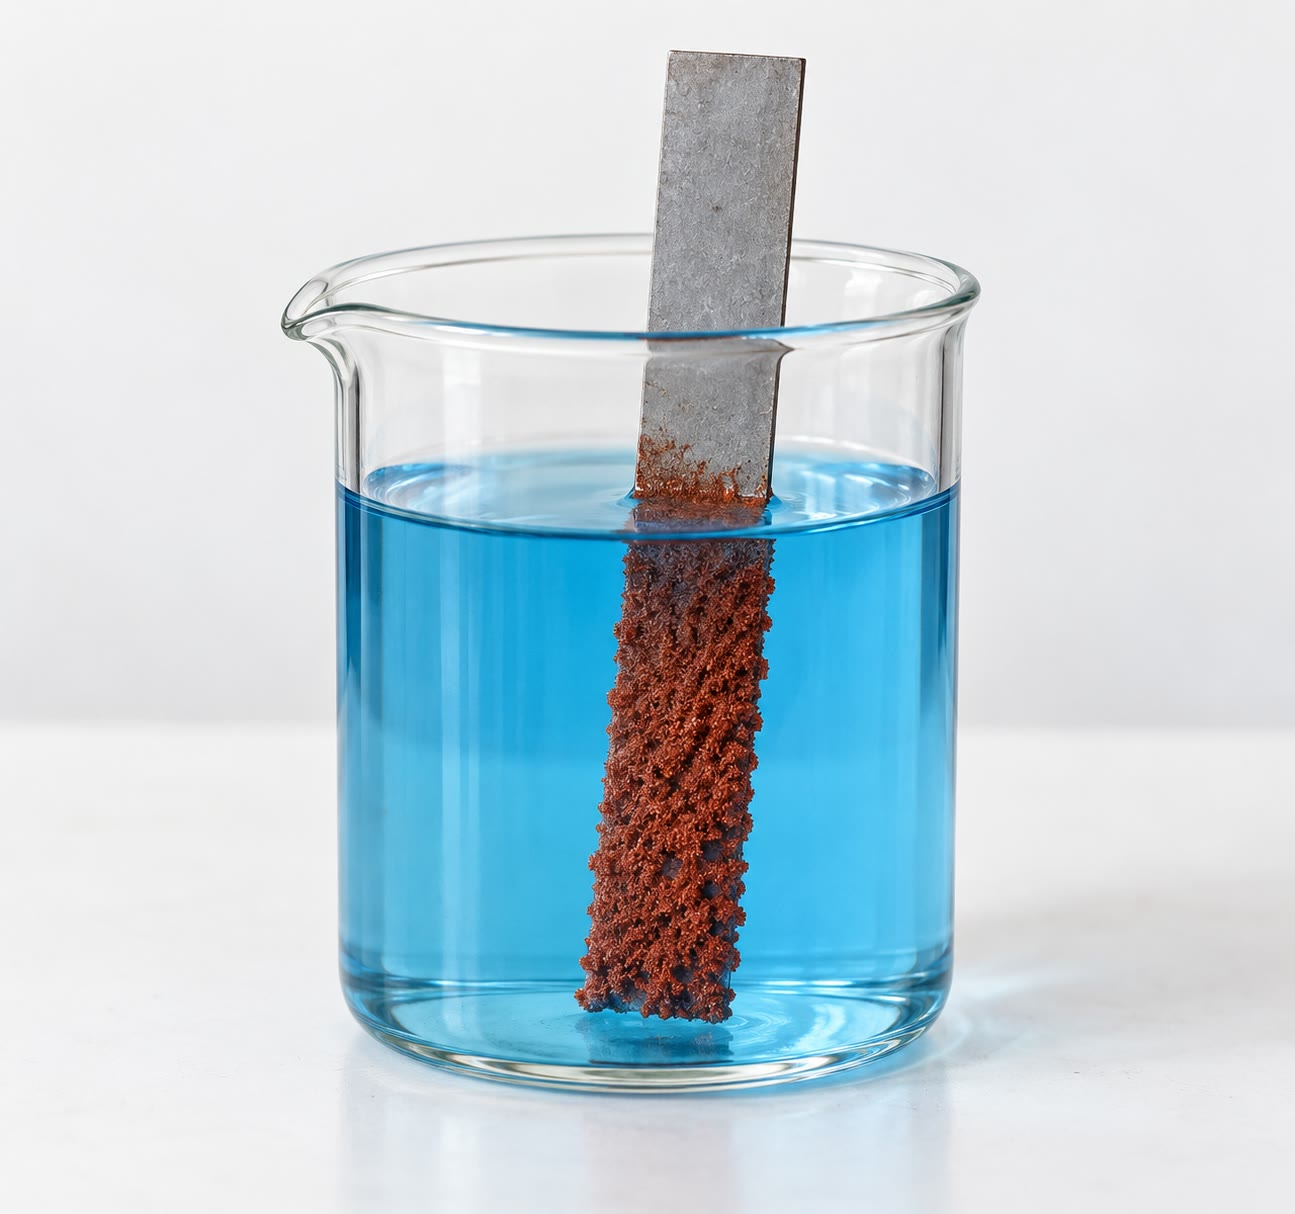
\includegraphics[width=0.55\linewidth]{images/book1/ai/g11-zinc-copper-sulfate.jpg}

{\small صفيحة خارصين في \omterm{def:g2:mixing-and-dissolving:dissolve}{محلول} كبريتات النحاس: يترسب النحاس على
الخارصين، وتحل \omterm{def:g9:ions:ion}{أيونات} الخارصين محله في \omterm{def:g2:mixing-and-dissolving:dissolve}{المحلول}.}
\end{omfigure}

\section{المؤكسدات والمختزلات}

\begin{definition}[المؤكسد والمختزل]\label{def:g11:redox:oxidant}
\emph{المؤكسد}\index{مؤكسد} \omterm{def:g6:pure-substances-and-mixtures:species}{نوع كيميائي} قادر على اكتساب \omterm{def:g9:inside-the-atom:nucleus}{إلكترون} أو
أكثر. و\emph{المختزل}\index{مختزل} \omterm{def:g6:pure-substances-and-mixtures:species}{نوع كيميائي} قادر على
التخلي عن \omterm{def:g9:inside-the-atom:nucleus}{إلكترون} أو أكثر.
\end{definition}

\begin{definition}[الأكسدة والاختزال]\label{def:g11:redox:oxidation}
\emph{الأكسدة}\index{أكسدة} فقد \omterm{def:g9:inside-the-atom:nucleus}{إلكترونات}؛
و\emph{الاختزال}\index{اختزال} اكتساب \omterm{def:g9:inside-the-atom:nucleus}{إلكترونات}. \omterm{def:g11:redox:oxidant}{فالمختزل}
يتأكسد، \omterm{def:g11:redox:oxidant}{والمؤكسد} يُختزل.
\end{definition}

\begin{remark}[طريقة للتذكر]\label{rem:g11:redox:remember}
في \emph{\omterm{def:g11:redox:oxidation}{الاختزال}} تُختزل شحنة \omterm{def:g6:pure-substances-and-mixtures:species}{النوع الكيميائي}: \omterm{def:g9:ions:ion}{فالأيون} \ce{Cu^{2+}}
يكتسب إلكترونين فيصير \ce{Cu}، والشحنة $+2 \to 0$. وفي
\omterm{def:g11:redox:oxidation}{الأكسدة} ترتفع الشحنة: \ce{Zn -> Zn^{2+} + 2e-}، $0 \to +2$.
\end{remark}

\begin{definition}[مزدوجة الأكسدة والاختزال ونصف المعادلة]\label{def:g11:redox:couple}
يكوّن \omterm{def:g11:redox:oxidant}{المؤكسد} \omterm{def:g11:redox:oxidant}{والمختزل} الذي يصير إليه باكتساب \omterm{def:g9:inside-the-atom:nucleus}{الإلكترونات}
\emph{مزدوجة أكسدة واختزال}\index{مزدوجة أكسدة واختزال}، تُكتب Ox/Red \omterm{def:g11:redox:oxidant}{والمؤكسد}
أولًا: $\ce{Cu^{2+}}/\ce{Cu}$، $\ce{Zn^{2+}}/\ce{Zn}$. ويوصف تبادل
\omterm{def:g9:inside-the-atom:nucleus}{الإلكترونات} داخل المزدوجة بما يسمى \emph{نصف المعادلة}\index{نصف معادلة} الخاصة بها،
\[
  \text{Ox} + n\,\ce{e-} \ce{<=>} \text{Red}, % ce-unbalanced-ok (generic form)
\]
موزونةً في \omterm{def:g7:atoms-and-molecules:atom}{الذرات} وفي الشحنة، مثلًا
\ce{Cu^{2+}(aq) + 2e- <=> Cu(s)}. ويدل السهم المزدوج على أن
التبادل يمكن أن يجري في الاتجاهين.
\end{definition}

\begin{example}[الفلزات وأيوناتها]\label{ex:g11:redox:metals}
كل \omterm{def:g9:periodic-table-first-look:metal}{فلز} يكوّن مزدوجة مع أيونه:
\begin{center}
\begin{tabular}{ll}
\hline
المزدوجة & \omterm{def:g11:redox:couple}{نصف المعادلة} \\
\hline
$\ce{Ag+}/\ce{Ag}$ & \ce{Ag+ + e- <=> Ag} \\
$\ce{Cu^{2+}}/\ce{Cu}$ & \ce{Cu^{2+} + 2e- <=> Cu} \\
$\ce{Fe^{2+}}/\ce{Fe}$ & \ce{Fe^{2+} + 2e- <=> Fe} \\
$\ce{Zn^{2+}}/\ce{Zn}$ & \ce{Zn^{2+} + 2e- <=> Zn} \\
$\ce{Al^{3+}}/\ce{Al}$ & \ce{Al^{3+} + 3e- <=> Al} \\
\hline
\end{tabular}
\end{center}
\omterm{def:g9:ions:ion}{والأيونات} أيضًا تكوّن مزدوجات: \ce{Fe^{3+} + e- <=> Fe^{2+}} للمزدوجة
$\ce{Fe^{3+}}/\ce{Fe^{2+}}$، و\ce{I2 + 2e- <=> 2I-} للمزدوجة
$\ce{I2}/\ce{I-}$. وكذلك الهيدروجين: \ce{2H+ + 2e- <=> H2} للمزدوجة
$\ce{H+}/\ce{H2}$.
\end{example}

\begin{remark}[نوع واحد، دوران]\label{rem:g11:redox:amphoteric}
يمكن \omterm{def:g6:pure-substances-and-mixtures:species}{لنوع كيميائي} أن يكون \omterm{def:g11:redox:oxidant}{مختزل} مزدوجة \omterm{def:g11:redox:oxidant}{ومؤكسد} مزدوجة أخرى.
\omterm{def:g9:ions:ion}{فالأيون} \ce{Fe^{2+}} هو \omterm{def:g11:redox:oxidant}{مؤكسد} المزدوجة $\ce{Fe^{2+}}/\ce{Fe}$ \omterm{def:g11:redox:oxidant}{ومختزل}
المزدوجة $\ce{Fe^{3+}}/\ce{Fe^{2+}}$. ويتوقف الدور الذي يؤديه على
شريكه في التفاعل.
\end{remark}

\section{تفاعلات الأكسدة والاختزال}

\begin{definition}[تفاعل الأكسدة والاختزال]\label{def:g11:redox:reaction}
\emph{تفاعل الأكسدة والاختزال}\index{تفاعل أكسدة واختزال} انتقال \omterm{def:g9:inside-the-atom:nucleus}{للإلكترونات}
من \omterm{def:g11:redox:oxidant}{مختزل} مزدوجة إلى \omterm{def:g11:redox:oxidant}{مؤكسد} مزدوجة أخرى. فيتأكسد
\omterm{def:g11:redox:oxidant}{المختزل} ويُختزل \omterm{def:g11:redox:oxidant}{المؤكسد}، في الوقت نفسه.
\end{definition}

\begin{proposition}[لا إلكترونات حرة]\label{prop:g11:redox:no-free-electrons}
لا توجد \omterm{def:g9:inside-the-atom:nucleus}{الإلكترونات} حرة في \omterm{def:g2:mixing-and-dissolving:dissolve}{المحلول}: فكل \omterm{def:g9:inside-the-atom:nucleus}{إلكترون} يعطيه
\omterm{def:g11:redox:oxidant}{المختزل} يأخذه \omterm{def:g11:redox:oxidant}{المؤكسد}. لذلك تُستنتج معادلة \omterm{def:g11:redox:reaction}{تفاعل الأكسدة والاختزال}
بجمع نصفي المعادلتين، بعد ضرب كل منهما في العدد الذي يجعل \omterm{def:g9:inside-the-atom:nucleus}{الإلكترونات}
المعطاة مساوية \omterm{def:g9:inside-the-atom:nucleus}{للإلكترونات} المأخوذة؛ فتُحذف \omterm{def:g9:inside-the-atom:nucleus}{الإلكترونات} عندئذ من الطرفين ولا تظهر في
المعادلة.
\end{proposition}

\begin{example}[الخارصين وأيونات النحاس]\label{ex:g11:redox:zinc-copper}
في المشهد الافتتاحي يتأكسد الخارصين وتُختزل \omterm{def:g9:ions:ion}{أيونات}
النحاس:
\[
\begin{array}{l@{\qquad}l}
  \ce{Zn(s) -> Zn^{2+}(aq) + 2e-} & \text{(أكسدة)}\\
  \ce{Cu^{2+}(aq) + 2e- -> Cu(s)} & \text{(اختزال)}\\
  \hline
  \ce{Zn(s) + Cu^{2+}(aq) -> Zn^{2+}(aq) + Cu(s)} &
\end{array}
\]
ينتقل إلكترونان من كل \omterm{def:g7:atoms-and-molecules:atom}{ذرة} خارصين إلى \omterm{def:g9:ions:ion}{أيون} نحاس واحد. واللون الأزرق
\omterm{def:g2:mixing-and-dissolving:dissolve}{للمحلول} هو لون \omterm{def:g9:ions:ion}{أيونات} \ce{Cu^{2+}}؛ ويبهت كلما استُهلكت،
بينما تحل محلها \omterm{def:g9:ions:ion}{أيونات} \ce{Zn^{2+}} عديمة
اللون.
\end{example}

\begin{omfigure}
\begin{tikzpicture}[font=\small, >=Stealth,
    ion/.style={circle, draw=black!70, minimum size=10mm, inner sep=0pt}]
  % the zinc strip and the solution
  \fill[black!18] (0,0) rectangle (1.6,4);
  \draw[black!60] (1.6,0) -- (1.6,4);
  \node[anchor=south] at (0.8,0.08) {خارصين};
  \fill[omWater!60] (1.6,0) rectangle (9.0,4);
  \node[anchor=north east] at (8.95,3.95) {محلول};
  % a zinc atom leaves as an ion
  \node[ion, fill=black!30] (zn) at (1.15,3.0) {\ce{Zn}};
  \node[ion, fill=white] (znion) at (5.0,3.0) {\ce{Zn^{2+}}};
  \draw[->, thick, omProp] (zn.east) -- (znion.west)
    node[midway, above] {أكسدة};
  % the electrons travel through the metal
  \draw[->, thick, omDef, dashed] (0.75,2.45) -- (0.75,1.55)
    node[midway, right] {2\,\ce{e-}};
  % a copper ion is reduced on the surface
  \node[ion, fill=omDef!35] (cuion) at (5.0,1.0) {\ce{Cu^{2+}}};
  \node[ion, fill=orange!55!brown] (cu) at (2.12,1.0) {\ce{Cu}};
  \draw[->, thick, omProp] (cuion.west) -- (cu.east)
    node[midway, above] {اختزال};
  \node[anchor=west, align=left] at (6.1,2.0) {كل ذرة خارصين\\ تعطي إلكترونين\\ لأيون نحاس واحد};
\end{tikzpicture}

{\small عند سطح الخارصين. تفقد \omterm{def:g7:atoms-and-molecules:atom}{ذرة} خارصين إلكترونين
وتغادر أيونًا \ce{Zn^{2+}}؛ وينتقل الإلكترونان عبر \omterm{def:g9:periodic-table-first-look:metal}{الفلز}
إلى \omterm{def:g9:ions:ion}{أيون} \ce{Cu^{2+}} يلامس السطح، فيصير \omterm{def:g7:atoms-and-molecules:atom}{ذرة} نحاس
ويبقى على الصفيحة.}
\end{omfigure}

\begin{omfigure}
\begin{tikzpicture}[font=\small]
  \pic at (0,0) {beaker={0.75}{omDef!45}};
  \fill[black!35] (-0.15,0.25) rectangle (0.15,2.5);
  \draw[black!65] (-0.15,0.25) rectangle (0.15,2.5);
  \node[anchor=north, align=center] at (0,-0.15) {في البداية:\\ \foreignlanguage{arabic}{محلول \ce{Cu^{2+}} أزرق}};
  \draw[->, thick, omProp] (1.3,1) -- (3.2,1) node[midway, above] {ساعة};
  \pic at (4.5,0) {beaker={0.75}{omDef!12}};
  \fill[black!35] (4.35,0.25) rectangle (4.65,2.5);
  \fill[orange!55!brown] (4.3,0.25) rectangle (4.7,1.5);
  \draw[black!65] (4.35,0.25) rectangle (4.65,2.5);
  \node[anchor=north, align=center] at (4.5,-0.15) {لاحقًا: محلول أبهت،\\ ونحاس على الخارصين};
\end{tikzpicture}

{\small ما يُرى: ترسب النحاس على الجزء المغمور من
الصفيحة، وبهتان اللون الأزرق \omterm{def:g9:ions:ion}{لأيونات} \ce{Cu^{2+}}.}
\end{omfigure}

\begin{example}[الفلزات في الحمض، من جديد]\label{ex:g11:redox:acid}
حين \omterm{def:g2:mixing-and-dissolving:dissolve}{يذوب} الحديد في حمض الهيدروكلوريك، يتأكسد الحديد
وتُختزل \omterm{def:g9:ions:ion}{أيونات} \ce{H+} إلى هيدروجين:
\[
  \ce{Fe(s) + 2H+(aq) -> Fe^{2+}(aq) + H2(g)}.
\]
والمزدوجتان هما $\ce{Fe^{2+}}/\ce{Fe}$ و$\ce{H+}/\ce{H2}$؛ أما \omterm{def:g9:ions:ion}{أيونات}
الكلوريد فلا تشارك.
\end{example}

\begin{inthelab}[شجرة الفضة]
تُعلَّق لفّة من سلك نحاس نظيف في كأس فيها \omterm{def:g2:mixing-and-dissolving:dissolve}{محلول} مخفف من نترات الفضة،
\ce{Ag+(aq) + NO3^-(aq)}. وفي غضون ساعة تنمو على طول السلك إبر متفرعة من
الفضة اللامعة، ويصير \omterm{def:g2:mixing-and-dissolving:dissolve}{المحلول} العديم اللون أزرق
باهتًا: \ce{Cu(s) + 2Ag+(aq) -> Cu^{2+}(aq) + 2Ag(s)}. ويجري
المعلم التجربة، بقفازين ونظارتين واقيتين، ويُجمع
\omterm{def:g2:mixing-and-dissolving:dissolve}{المحلول} بعدها نفاياتٍ خطرة.
\end{inthelab}

\begin{safety}{\ghs[0.82cm]{GHS03}\ghs[0.82cm]{GHS05}\ghs[0.82cm]{GHS08}\ghs[0.82cm]{GHS09}}
% ledger: ghs:AgNO3
نترات الفضة: \omterm{def:g11:redox:oxidant}{مؤكسد} قد يغذي حريقًا (GHS03)؛ أكّال للجلد
والعينين، ويصبغ الجلد بالأسود (GHS05)؛ خطر على الصحة
(GHS08)؛ شديد السمية للأحياء المائية، فلا يُسكب أبدًا في المغسلة
(GHS09).
\end{safety}

\begin{omfigure}
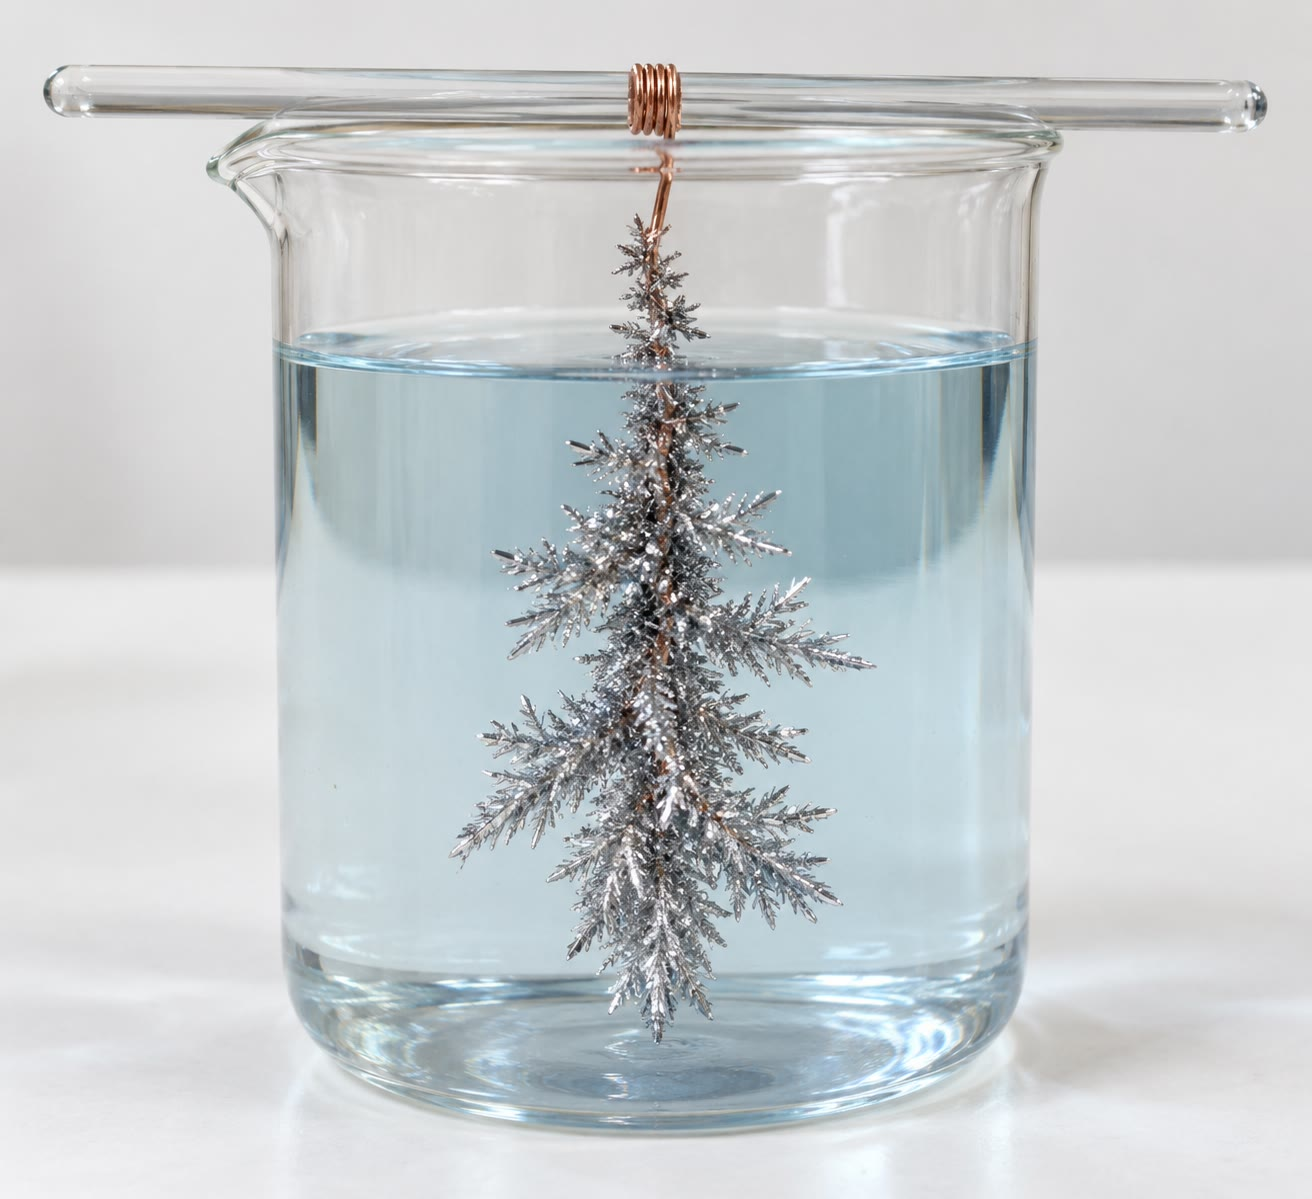
\includegraphics[width=0.5\linewidth]{images/book1/ai/g11-silver-tree.jpg}

{\small بلورات فضة تنمو على سلك نحاس في \omterm{def:g2:mixing-and-dissolving:dissolve}{محلول} نترات
الفضة.}
\end{omfigure}

\section{موازنة أنصاف المعادلات}

كثير من المزدوجات المهمة تحوي الأكسجين وتُكتب للمحاليل
الحمضية، حيث توجد \omterm{def:g9:ions:ion}{أيونات} \ce{H+}. وتحتاج أنصاف معادلاتها إلى
\omterm{def:g7:atoms-and-molecules:molecule}{جزيئات} ماء \omterm{def:g9:ions:ion}{وأيونات} \ce{H+} لكي تتوازن.

\begin{method}[موازنة نصف معادلة في محلول حمضي]\label{met:g11:redox:balance}
لكتابة \omterm{def:g11:redox:couple}{نصف معادلة} المزدوجة Ox/Red في \omterm{def:g9:acids-bases-ph:acidic}{محلول حمضي}:
\begin{enumerate}
  \item اكتب Ox على اليسار وRed على اليمين، ووازن \omterm{def:g7:atoms-and-molecules:atom}{الذرة}
        التي ليست O ولا H؛
  \item وازن \omterm{def:g7:atoms-and-molecules:atom}{ذرات} الأكسجين \omterm{def:g7:atoms-and-molecules:molecule}{بجزيئات} الماء \ce{H2O}؛
  \item وازن \omterm{def:g7:atoms-and-molecules:atom}{ذرات} الهيدروجين \omterm{def:g9:ions:ion}{بأيونات} \ce{H+}؛
  \item وازن الشحنة \omterm{def:g9:inside-the-atom:nucleus}{بالإلكترونات} \ce{e-}، على اليسار؛
  \item تحقق: العدد نفسه من كل \omterm{def:g7:atoms-and-molecules:atom}{ذرة}، والشحنة الكلية نفسها في
        الطرفين.
\end{enumerate}
\end{method}

\begin{example}[أيون البرمنغنات]\label{ex:g11:redox:permanganate}
للمزدوجة $\ce{MnO4^-}/\ce{Mn^{2+}}$ (من البنفسجي الداكن إلى عديم اللون
تقريبًا): المنغنيز موزون؛ وأربع \omterm{def:g7:atoms-and-molecules:atom}{ذرات} O على اليسار تعطي
$\ce{4H2O}$ على اليمين؛ \omterm{def:g7:atoms-and-molecules:atom}{وذرات} H الثماني فيها تعطي $\ce{8H+}$ على اليسار؛
والشحنة على اليسار $-1 + 8 = +7$، وعلى اليمين $+2$، فتُضاف خمسة
\omterm{def:g9:inside-the-atom:nucleus}{إلكترونات} على اليسار:
\[
  \ce{MnO4^-(aq) + 8H+(aq) + 5e- <=> Mn^{2+}(aq) + 4H2O(l)}.
\]
\end{example}

\begin{example}[أيون ثنائي الكرومات]\label{ex:g11:redox:dichromate}
للمزدوجة $\ce{Cr2O7^{2-}}/\ce{Cr^{3+}}$ (من البرتقالي إلى الأخضر): ذرتا كروم على
اليمين؛ وسبع \omterm{def:g7:atoms-and-molecules:atom}{ذرات} O تعطي \ce{7H2O}؛ وأربع عشرة \omterm{def:g7:atoms-and-molecules:atom}{ذرة} H تعطي \ce{14H+}؛ والشحنة
$-2 + 14 = +12$ على اليسار مقابل $2 \times 3 = +6$ على اليمين، فتُضاف
ستة \omterm{def:g9:inside-the-atom:nucleus}{إلكترونات}:
\[
  \ce{Cr2O7^{2-}(aq) + 14H+(aq) + 6e- <=> 2Cr^{3+}(aq) + 7H2O(l)}.
\]
\end{example}

\begin{method}[كتابة معادلة أكسدة واختزال]\label{met:g11:redox:combine}
لكتابة معادلة التفاعل بين \omterm{def:g11:redox:oxidant}{المؤكسد} Ox$_1$ لمزدوجة
\omterm{def:g11:redox:oxidant}{والمختزل} Red$_2$ لمزدوجة أخرى:
\begin{enumerate}
  \item اكتب نصفي المعادلتين، الأول في اتجاه
        \omterm{def:g11:redox:oxidation}{الاختزال} (Ox$_1 \to$ Red$_1$)، والثاني في اتجاه
        \omterm{def:g11:redox:oxidation}{الأكسدة} (Red$_2 \to$ Ox$_2$)؛
  \item اضربهما في أصغر عددين يجعلان \omterm{def:g9:inside-the-atom:nucleus}{الإلكترونات}
        متساوية؛
  \item اجمعهما؛ فتُحذف \omterm{def:g9:inside-the-atom:nucleus}{الإلكترونات}، وقد يُحذف كذلك بعض \ce{H+}
        و\ce{H2O} مما يظهر في الطرفين؛
  \item تحقق من \omterm{def:g7:atoms-and-molecules:atom}{الذرات} والشحنة مرة أخرى.
\end{enumerate}
\end{method}

\begin{example}[البرمنغنات والحديد (II)]\label{ex:g11:redox:mno4-fe}
يؤكسد \omterm{def:g9:ions:ion}{أيون} البرمنغنات \omterm{def:g9:ions:ion}{أيونات} \ce{Fe^{2+}} إلى \ce{Fe^{3+}}:
\[
\begin{array}{l@{\qquad}l}
  \ce{MnO4^- + 8H+ + 5e- -> Mn^{2+} + 4H2O} & \times 1\\
  \ce{Fe^{2+} -> Fe^{3+} + e-} & \times 5\\
  \hline
  \ce{MnO4^- + 8H+ + 5Fe^{2+} -> Mn^{2+} + 5Fe^{3+} + 4H2O} &
\end{array}
\]
الشحنة على اليسار: $-1 + 8 + 10 = +17$؛ وعلى اليمين: $2 + 15 = +17$.
ويُستعمل هذا التفاعل في الفصل التالي لقياس كمية من
الحديد (II).
\end{example}

\section{مؤكسدات ومختزلات من حولنا}

\begin{proposition}[بعض المؤكسدات والمختزلات الشائعة]\label{prop:g11:redox:common}
نلقى الأنواع الكيميائية الآتية مرة بعد مرة في المختبر وفي
الحياة اليومية:
\begin{center}
\small
\begin{tabular}{lll}
\hline
\omterm{def:g6:pure-substances-and-mixtures:species}{النوع الكيميائي} & الدور & \omterm{def:g11:redox:couple}{نصف معادلة} مزدوجته \\
\hline
ثنائي الأكسجين \ce{O2} & \omterm{def:g11:redox:oxidant}{مؤكسد} & \ce{O2 + 4H+ + 4e- <=> 2H2O} \\
ثنائي الكلور \ce{Cl2} & \omterm{def:g11:redox:oxidant}{مؤكسد} & \ce{Cl2 + 2e- <=> 2Cl-} \\
تحت الكلوريت \ce{ClO-} (ماء جافيل) & \omterm{def:g11:redox:oxidant}{مؤكسد} & \ce{2ClO- + 4H+ + 2e- <=> Cl2 + 2H2O} \\
بيروكسيد الهيدروجين \ce{H2O2} & \omterm{def:g11:redox:oxidant}{مؤكسد} & \ce{H2O2 + 2H+ + 2e- <=> 2H2O} \\
البرمنغنات \ce{MnO4^-} & \omterm{def:g11:redox:oxidant}{مؤكسد} & \ce{MnO4^- + 8H+ + 5e- <=> Mn^{2+} + 4H2O} \\
\omterm{def:g9:periodic-table-first-look:metal}{الفلزات} \ce{M} (\ce{Fe}، \ce{Zn}، \ce{Al}\dots) & مختزلات & \ce{M^{n+} + $n$ e- <=> M} % ce-unbalanced-ok (generic)
\\
اليوديد \ce{I-} & \omterm{def:g11:redox:oxidant}{مختزل} & \ce{I2 + 2e- <=> 2I-} \\
الثيوكبريتات \ce{S2O3^{2-}} & \omterm{def:g11:redox:oxidant}{مختزل} & \ce{S4O6^{2-} + 2e- <=> 2S2O3^{2-}} \\
حمض الأسكوربيك \ce{C6H8O6} (فيتامين C) & \omterm{def:g11:redox:oxidant}{مختزل} & \ce{C6H6O6 + 2H+ + 2e- <=> C6H8O6} \\
\hline
\end{tabular}
\end{center}
\end{proposition}

\begin{example}[النحاس يخضرّ]\label{ex:g11:redox:patina}
السطوح والتماثيل النحاسية المتروكة في \omterm{def:g4:air-a-mixture-of-gases:air}{الهواء} الطلق عقودًا تخضرّ ببطء
خضرةً باهتة. فأكسجين \omterm{def:g4:air-a-mixture-of-gases:air}{الهواء} يؤكسد النحاس إلى \omterm{def:g9:ions:ion}{أيونات} \ce{Cu^{2+}}،
تكوّن مع الماء وثنائي أكسيد الكربون قشرة خضراء رقيقة هي
الزنجار. وخلافًا \omterm{def:g9:metals-acids-corrosion:corrosion}{لصدأ} الحديد، يلتصق الزنجار \omterm{def:g9:periodic-table-first-look:metal}{بالفلز}
ويحميه من أي هجوم لاحق.
\end{example}

\begin{omfigure}

\includegraphics[width=0.48\linewidth]{images/book1/ai/g11-green-roof.jpg}

{\small سطح نحاسي بعد عقود في \omterm{def:g4:air-a-mixture-of-gases:air}{الهواء}: النحاس \omterm{def:g11:redox:oxidant}{المؤكسد} يكوّن
زنجارًا أخضر.}
\end{omfigure}

\begin{remark}[مضادات الأكسدة]\label{rem:g11:redox:antioxidant}
«مضاد \omterm{def:g11:redox:oxidation}{الأكسدة}» المضاف إلى الغذاء \omterm{def:g11:redox:oxidant}{مختزل} يؤكسده
أكسجين \omterm{def:g4:air-a-mixture-of-gases:air}{الهواء} قبل أن يؤكسد الغذاء. وفيتامين C (حمض الأسكوربيك) أشيعها:
فتفاحة مقطوعة رُشّ عليها عصير الليمون تسمرّ أبطأ بكثير،
لأن فيتامين C في الليمون يتأكسد أولًا.
\end{remark}

\section{تمارين}

\begin{exercise}[$\star$]\label{exo:g11:redox:1}
عرّف \omterm{def:g11:redox:oxidant}{المؤكسد}، \omterm{def:g11:redox:oxidant}{والمختزل}، \omterm{def:g11:redox:oxidation}{والأكسدة}، \omterm{def:g11:redox:oxidation}{والاختزال}.
\end{exercise}

\begin{exercise}[$\star$]\label{exo:g11:redox:2}
اكتب لكل زوج مزدوجة \omterm{def:g11:redox:oxidation}{الأكسدة} \omterm{def:g11:redox:oxidation}{والاختزال} بالشكل Ox/Red: \ce{Fe}
و\ce{Fe^{2+}}؛ و\ce{Ag} و\ce{Ag+}؛ و\ce{I-} و\ce{I2}؛ و\ce{Fe^{2+}}
و\ce{Fe^{3+}}.
\end{exercise}

\begin{exercise}[$\star$]\label{exo:g11:redox:3}
اكتب أنصاف معادلات المزدوجات $\ce{Ag+}/\ce{Ag}$،
و$\ce{Al^{3+}}/\ce{Al}$، و$\ce{Fe^{3+}}/\ce{Fe^{2+}}$، و$\ce{Cl2}/\ce{Cl-}$.
\end{exercise}

\begin{exercise}[$\star$]\label{exo:g11:redox:4}
أيمثل التحول \ce{Fe -> Fe^{2+} + 2e-} \omterm{def:g11:redox:oxidation}{أكسدة} أم
اختزالًا؟ وهل يسلك الحديد سلوك \omterm{def:g11:redox:oxidant}{مؤكسد} أم \omterm{def:g11:redox:oxidant}{مختزل}؟
\end{exercise}

\begin{exercise}[$\star$]\label{exo:g11:redox:5}
في التفاعل \ce{Zn + Cu^{2+} -> Zn^{2+} + Cu}، سمِّ \omterm{def:g6:pure-substances-and-mixtures:species}{النوع الكيميائي}
الذي يتأكسد، والنوع الذي يُختزل، \omterm{def:g11:redox:oxidant}{والمؤكسد}، \omterm{def:g11:redox:oxidant}{والمختزل}، وأعطِ
عدد \omterm{def:g9:inside-the-atom:nucleus}{الإلكترونات} المنتقلة لكل \omterm{def:g7:atoms-and-molecules:atom}{ذرة} خارصين.
\end{exercise}

\begin{exercise}[$\star\star$]\label{exo:g11:redox:6}
وازن، في \omterm{def:g9:acids-bases-ph:acidic}{محلول حمضي}، \omterm{def:g11:redox:couple}{نصف معادلة} المزدوجة
$\ce{H2O2}/\ce{H2O}$، متبعًا \cref{met:g11:redox:balance} خطوةً
خطوةً.
\end{exercise}

\begin{exercise}[$\star\star$]\label{exo:g11:redox:7}
اكتب معادلة التفاعل بين ثنائي اليود \ce{I2} \omterm{def:g9:ions:ion}{وأيون}
الثيوكبريتات \ce{S2O3^{2-}}، الذي يعطي \omterm{def:g9:ions:ion}{أيونات} اليوديد \omterm{def:g9:ions:ion}{وأيونات}
رباعي الثيونات \ce{S4O6^{2-}}.
\end{exercise}

\begin{exercise}[$\star\star$]\label{exo:g11:redox:8}
اكتب معادلة تفاعل شجرة الفضة انطلاقًا من نصفي
معادلتيه، واشرح لماذا يصير \omterm{def:g2:mixing-and-dissolving:dissolve}{المحلول} أزرق.
\end{exercise}

\begin{exercise}[$\star\star$]\label{exo:g11:redox:9}
يتفاعل فيتامين C، \ce{C6H8O6}، مع ثنائي اليود \ce{I2}. اكتب معادلة
التفاعل، وبيّن أي النوعين هو \omterm{def:g11:redox:oxidant}{المختزل}.
\end{exercise}

\begin{exercise}[$\star\star$]\label{exo:g11:redox:10}
يتفاعل الألومنيوم مع \omterm{def:g9:ions:ion}{أيونات} النحاس (II). اكتب المعادلة، واشرح
لماذا يجب ضرب نصفي المعادلتين في 2 وفي 3.
\end{exercise}

\begin{exercise}[$\star\star$]\label{exo:g11:redox:11}
يؤكسد بيروكسيد الهيدروجين \omterm{def:g9:ions:ion}{أيونات} الحديد (II) إلى \omterm{def:g9:ions:ion}{أيونات} الحديد (III) في \omterm{def:g9:acids-bases-ph:acidic}{محلول
حمضي}. اكتب المعادلة.
\end{exercise}

\begin{exercise}[$\star\star\star$]\label{exo:g11:redox:12}
تفقد صفيحة خارصين \qty{1.30}{g} في \omterm{def:g2:mixing-and-dissolving:dissolve}{محلول} يحوي فائضًا من
\omterm{def:g9:ions:ion}{أيونات} النحاس (II). ما كتلة النحاس المترسبة؟ خذ
$M(\ce{Zn}) = \qty{65.4}{g/mol}$ و$M(\ce{Cu}) = \qty{63.5}{g/mol}$.
\end{exercise}

\begin{exercise}[$\star\star\star$]\label{exo:g11:redox:13}
اكتب معادلة \omterm{def:g11:redox:oxidation}{أكسدة} \omterm{def:g9:ions:ion}{أيونات} الحديد (II) \omterm{def:g9:ions:ion}{بأيونات} ثنائي الكرومات
في \omterm{def:g9:acids-bases-ph:acidic}{محلول حمضي}. ما كمية \ce{Fe^{2+}} التي يؤكسدها
\qty{0.010}{mol} من \omterm{def:g9:ions:ion}{أيونات} ثنائي الكرومات؟
\end{exercise}

\begin{exercise}[$\star\star\star$]\label{exo:g11:redox:14}
يحوي ماء جافيل \omterm{def:g9:ions:ion}{أيونات} تحت الكلوريت \ce{ClO-} \omterm{def:g9:ions:ion}{وأيونات} الكلوريد
\ce{Cl-}. مستعينًا بالمزدوجتين $\ce{ClO-}/\ce{Cl2}$ و$\ce{Cl2}/\ce{Cl-}$،
اكتب معادلة التفاعل الذي يحدث حين يلتقي ماء جافيل
بحمض، واشرح لماذا تحذّر لصاقات ماء جافيل ولصاقات منتجات إزالة الكلس
الحمضية كلتاهما من خلطهما أبدًا.
\end{exercise}

\begin{exercise}[$\star\star\star$]\label{exo:g11:redox:15}
في شكل سطح الخارصين، تنتقل \omterm{def:g9:inside-the-atom:nucleus}{الإلكترونات} عبر
\omterm{def:g9:periodic-table-first-look:metal}{الفلز}، لا عبر \omterm{def:g2:mixing-and-dissolving:dissolve}{المحلول}. مستعينًا بما في \cref{prop:g11:redox:no-free-electrons}،
اشرح لماذا يترسب النحاس على صفيحة الخارصين نفسها لا
في موضع آخر من الكأس.
\end{exercise}

\section{مسألة: اختبار النَّفَس}

\begin{problem}[{مسألة نهاية الأسبوع --- كيمياء أنبوب كشف الكحول في
النَّفَس: مزدوجتان، وتغير لوني من البرتقالي إلى الأخضر، وكتلة الإيثانول
التي يستطيع الأنبوب كشفها، وخلية الوقود التي حلّت محله}]
\label{pb:g11:redox:1}
% ledger: ghs:K2Cr2O7, breath:ratio; molar masses from tools/molar_mass.py
% (0.1-rounded weights): K2Cr2O7 294.2, C2H6O 46.0 g/mol
استعملت أولى اختبارات \omterm{def:g11:functional-groups:alcohol}{الكحول} في النَّفَس أنبوبًا زجاجيًا مملوءًا بحبيبات من
السيليكا مغطاة بثنائي كرومات البوتاسيوم البرتقالي، \ce{K2Cr2O7}، في وسط حمضي.
فالإيثانول، \ce{CH3CH2OH}، الموجود في النَّفَس المنفوخ عبر الأنبوب يختزل
\omterm{def:g9:ions:ion}{أيونات} ثنائي الكرومات إلى \omterm{def:g9:ions:ion}{أيونات} \ce{Cr^{3+}} خضراء، ويتأكسد إلى حمض
الإيثانويك، \ce{CH3COOH}؛ وطول المنطقة الخضراء يقيس الإيثانول.
لنفترض أن أنبوبًا يحوي \qty{2.0}{mg} من ثنائي كرومات البوتاسيوم. استعمل
$M(\ce{K}) = 39.1$، و$M(\ce{Cr}) = 52.0$، و$M(\ce{O}) = 16.0$،
و$M(\ce{C}) = 12.0$، و$M(\ce{H}) = \qty{1.0}{g/mol}$، و$N_A =
\qty{6.02e23}{mol^{-1}}$ و$e = \qty{1.60e-19}{C}$.

\medskip
\noindent\textbf{الجزء الأول --- مزدوجتان.}
\begin{enumerate}
  \item سمِّ مزدوجتي \omterm{def:g11:redox:oxidation}{الأكسدة} \omterm{def:g11:redox:oxidation}{والاختزال} المعنيتين، \omterm{def:g11:redox:oxidant}{والمؤكسد} أولًا.
  \item أيتأكسد الإيثانول أم يُختزل؟ وهل هو \omterm{def:g11:redox:oxidant}{المؤكسد} أم
        \omterm{def:g11:redox:oxidant}{المختزل}؟
  \item اكتب \omterm{def:g11:redox:couple}{نصف معادلة} المزدوجة
        $\ce{Cr2O7^{2-}}/\ce{Cr^{3+}}$ في \omterm{def:g9:acids-bases-ph:acidic}{محلول حمضي}.
  \item اكتب \omterm{def:g11:redox:couple}{نصف معادلة} المزدوجة
        $\ce{CH3COOH}/\ce{CH3CH2OH}$ في \omterm{def:g9:acids-bases-ph:acidic}{محلول حمضي}.
  \item استنتج معادلة التفاعل في الأنبوب.
\end{enumerate}

\medskip
\noindent\textbf{الجزء الثاني --- ما يستطيع أنبوب واحد قياسه.}
\begin{enumerate}[resume]
  \item اشرح تغير لون الحبيبات.
  \item احسب \omterm{def:g10:the-mole:molar-mass}{الكتلة المولية} لثنائي كرومات البوتاسيوم.
  \item احسب كمية \omterm{def:g9:ions:ion}{أيونات} ثنائي الكرومات في الأنبوب.
  \item ما كمية الإيثانول اللازمة لتحويل الأنبوب كله إلى الأخضر؟
  \item استنتج أكبر كتلة من الإيثانول يستطيع أنبوب واحد قياسها.
\end{enumerate}

\medskip
\noindent\textbf{الجزء الثالث --- من النَّفَس إلى الدم.}
ينفخ شخص \qty{1.0}{L} من النَّفَس عبر الأنبوب؛ فتنمو المنطقة الخضراء
بما يتناسب مع كتلة الإيثانول التي تصل إليها.
\begin{enumerate}[resume]
  \item يحوي النَّفَس \qty{0.25}{mg} من الإيثانول في اللتر. ما
        الكسر المستهلك من ثنائي الكرومات؟
  \item طول الأنبوب \qty{10}{cm}. ما طول المنطقة الخضراء؟
  \item تفترض أجهزة تحليل النَّفَس أن \qty{2100}{L} من النَّفَس تحمل
        من الإيثانول قدر ما يحمله \qty{1}{L} من الدم. قدّر كتلة الإيثانول
        في لتر الدم، بالغرام.
  \item لماذا تبدأ المنطقة الخضراء عند مدخل الأنبوب وتنمو
        نحو مخرجه، بدل أن يخضرّ الأنبوب كله
        قليلًا؟
  \item لماذا لا يُستعمل الأنبوب إلا مرة واحدة؟
\end{enumerate}

\medskip
\noindent\textbf{الجزء الرابع --- خلية \omterm{def:g4:what-a-fire-needs:fuel}{الوقود}.}
يحمل ثنائي كرومات البوتاسيوم الرسوم التوضيحية
\ghs[0.6cm]{GHS03}\,\ghs[0.6cm]{GHS05}\,\ghs[0.6cm]{GHS06}\,\ghs[0.6cm]{GHS07}\,\ghs[0.6cm]{GHS08}\,\ghs[0.6cm]{GHS09}.
وتستعمل الأجهزة الحديثة بدلًا منه خلية \omterm{def:g4:what-a-fire-needs:fuel}{وقود}، يتأكسد فيها إيثانول
النَّفَس بثنائي الأكسجين على قطب، وتسري \omterm{def:g9:inside-the-atom:nucleus}{الإلكترونات}
المتحررة في سلك.
\begin{enumerate}[resume]
  \item أعطِ سببين، تقرؤهما من الرسوم التوضيحية، للتخلي عن أنابيب
        ثنائي الكرومات.
  \item اكتب معادلة \omterm{def:g11:redox:oxidation}{أكسدة} الإيثانول بثنائي الأكسجين،
        مستعينًا بالمزدوجة $\ce{O2}/\ce{H2O}$.
  \item كم إلكترونًا يتخلى عنه \omterm{def:g7:atoms-and-molecules:molecule}{جزيء} إيثانول واحد حين
        يتأكسد إلى حمض الإيثانويك؟
  \item احسب، لكتلة \qty{0.25}{mg} من الإيثانول، كمية الإيثانول،
        ثم عدد \omterm{def:g9:inside-the-atom:nucleus}{الإلكترونات} المتحررة.
  \item استنتج الشحنة الكهربائية التي تسري في خلية \omterm{def:g4:what-a-fire-needs:fuel}{الوقود}.
        ولماذا تُعد هذه الشحنة مقياسًا جيدًا للإيثانول في النَّفَس؟
\end{enumerate}
\end{problem}
